\title{STA 602 HW2}
\documentclass[11pt, letterpaper]{article}
\usepackage[utf8]{inputenc}
\usepackage[letterpaper, margin=0.5in]{geometry}
\usepackage{amsmath}
\usepackage{amssymb}
\usepackage{amsthm}
\usepackage{graphicx}
\usepackage[font=scriptsize]{caption}
\usepackage{subcaption}
\graphicspath{ {.} }
\captionsetup{justification=raggedright, singlelinecheck=false}

\author{Ryan Tang}
\date{October 7th 2022}

\begin{document}
\maketitle

\section{HW4 Exercise 3}
\paragraph{(d)}
Now instead of plotting MSE, here we estimated MAE using Monte Carlo. Still the exact 5 estimators, below are the MAE comparisons (Figures 5 and 6). The general Bayesian update behaviors stay directionally similar between L2 and L1. L1 is just sharper and rigid. Lastly, the $\delta_5$ L2 minimax estimator is still a minimax estimator in the L1 context.
\begin{figure*}[!h]
  \centering
  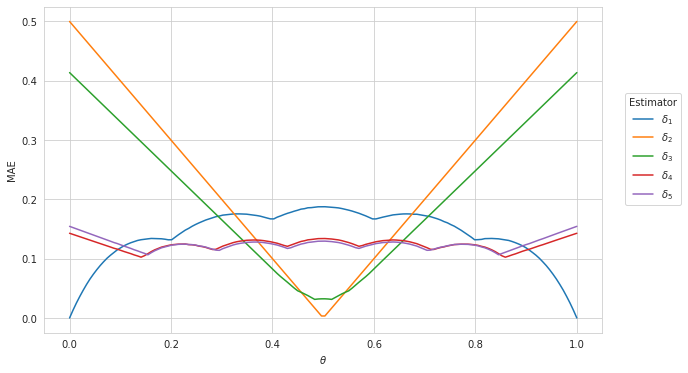
\includegraphics[width=0.7\textwidth]{3.d.1.png}
  \captionsetup{justification=centering}
  \caption{Political Poll MAE Comparison, $n = 5$}
\end{figure*}

\begin{figure*}[!h]
  \centering
  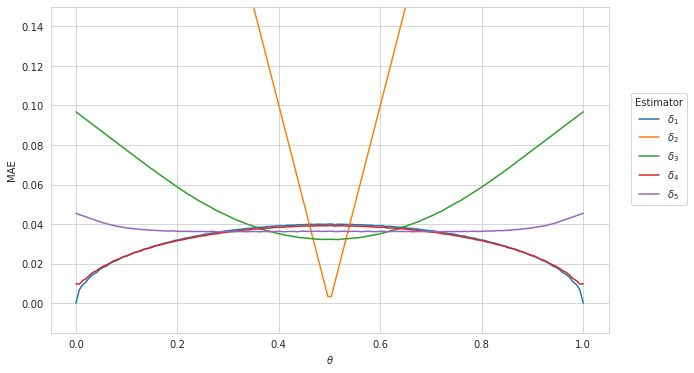
\includegraphics[width=0.7\textwidth]{3.d.2.png}
  \captionsetup{justification=centering}
  \caption{Political Poll MAE Comparison, $n = 100$}
\end{figure*}

\section{Exercise 4.1}
Based on Exercise 3.1, we have the following posterior for $\theta_1$. And assuming a uniform prior for $\theta_2$, a Binomial generating model for $Y_2$, and a sample of 50 with 30 supports for the policy, we can also write $\theta_2$'s posterior in Beta.
\begin{align*}
    \theta_1|Y_1 &\thicksim Beta(57+1, 1+100-57) = Beta(a=58, b=44) \\
    \theta_2|Y_2 &\thicksim Beta(30+1, 1+50-30) = Beta(a=31, b=21)
\end{align*}
Now, after some sampling with MC, we estimated $p(\theta_1 < \theta_2|Y_1, Y_2) = 0.6316$


\section{Exercise 4.2}
\paragraph{(a)}
According to Exercise 3.3, we have the following prior and posterior for groups $A$ and $B$.
\begin{align*}
    \theta_A &\thicksim Beta(120, 10) && \theta_A|\mathbf{y}_A \thicksim Beta(237, 20) \\
    \theta_B &\thicksim Beta(12, 1) && \theta_A|\mathbf{y}_B \thicksim Beta(125, 14)
\end{align*}
Hence, the estimated $p(\theta_B < \theta_A|\mathbf{y}_A, \mathbf{y}_B) = 0.9957$


\paragraph{(b)}
By adjusting the $\theta_B$ prior with the parameter, $n_0$. We can adjust how strong the prior belief is and make it more insensitive to the new survey data the higher it is. Below is a plot of the sensitivity. As we can see, with $n_0$ increases, the posterior $\{\theta_B < \theta_A\}$ stay closer to 50\%. 
\begin{figure*}[!h]
  \centering
  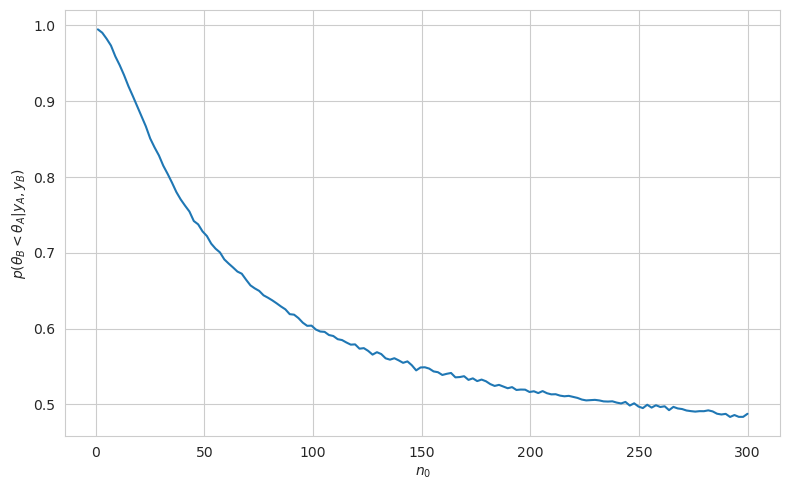
\includegraphics[width=0.7\textwidth]{4.2.b.png}
  \captionsetup{justification=centering}
  \caption{Sensitivity of $\{\theta_B < \theta_A\}$ with respect to $n_0$}
\end{figure*}

\paragraph{(c)}
Here we repeat the same thing done in (a) and (b) to the posterior predictive distribution. When we have $n_0=1$, we have $p(\tilde{Y}_B < \tilde{Y}_A|\mathbf{y}_A, \mathbf{y}_B) = 0.6969$. And below is the sensitivity with $n_0$. The higher the $n_0$, the stronger we believe that $\theta_B$ has a mean of 12, and the observed data will be less dominant in the posterior.

\begin{figure*}[!h]
  \centering
  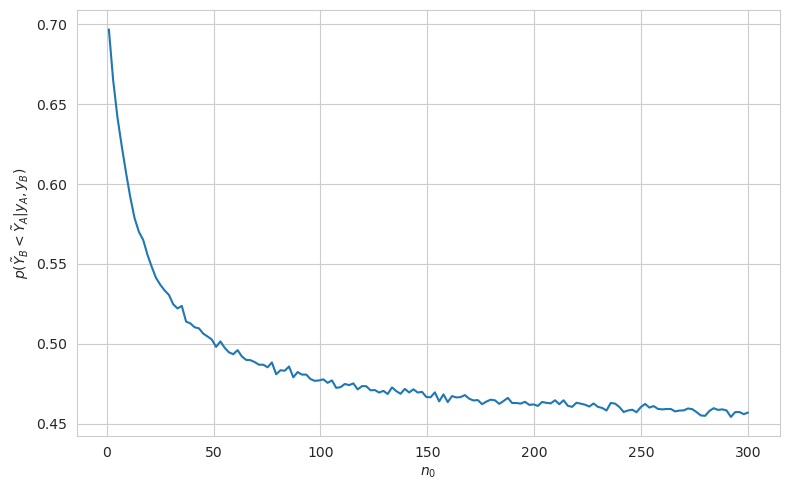
\includegraphics[width=0.7\textwidth]{4.2.c.png}
  \captionsetup{justification=centering}
  \caption{Sensitivity of $\{\tilde{Y}_B < \tilde{Y}_A\}$ with respect to $n_0$}
\end{figure*}

\section{Exercise 4.4}
\paragraph{(a)}
According to Exercise 3.4, we have a mixture of Beta prior for $\theta$ and a Binominal data generating model with $n=43, y=15$. Hence, the resulting posterior is still a beta mixture with an updated weight $w_i$ proportional to the new density. And its estimated 95\% confidence interval is $[0.2036, 0.4578]$.
\begin{align*}
    p(\theta) &\propto \frac{3}{4} \theta (1-\theta)^7 + \frac{1}{4} \theta^7(1-\theta) \\
    p(y|\theta) &\propto \theta^y \theta^{n-y} \\
    p(\theta|y) &\propto w_1 \theta^{16} (1-\theta)^{35} + w_2 \theta^{22}(1-\theta)^{29}
\end{align*}

\begin{figure*}[!h]
  \centering
  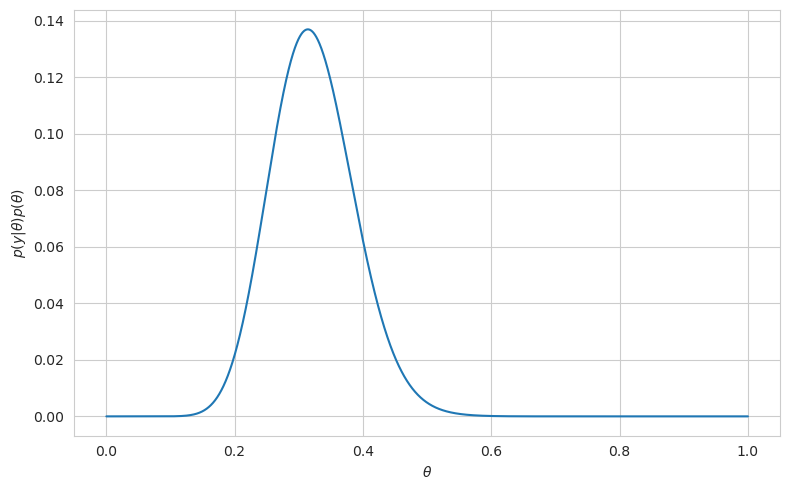
\includegraphics[width=0.7\textwidth]{4.4.a.png}
  \captionsetup{justification=centering}
  \caption{Posterior Kernel Estimation using Discrete Approximation}
\end{figure*}

\paragraph{(b)}
Since we have derived the weight for each Beta component $w1\approx0.985, w2\approx0.015$, we can generate the posterior samples through MC. Below is the density estimation of 1,000,000 posterior samples and the estimated 95\% confidence interval, [0.2037, 0.4580].

\begin{figure*}[!h]
  \centering
  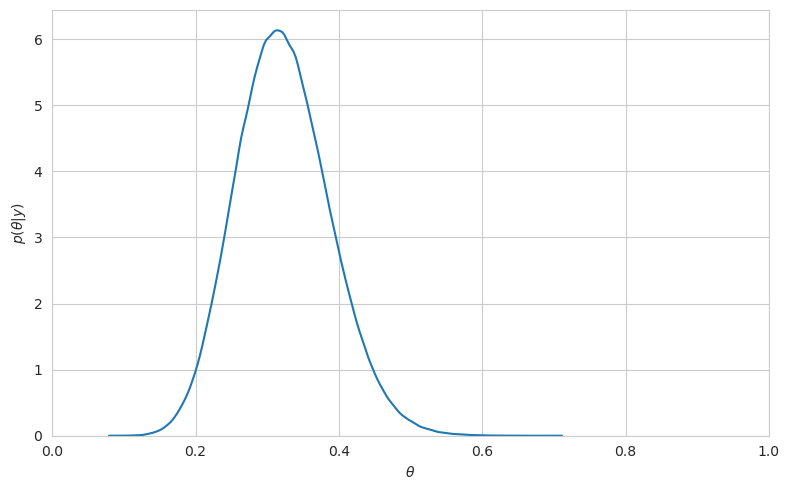
\includegraphics[width=0.7\textwidth]{4.4.b.png}
  \captionsetup{justification=centering}
  \caption{Posterior KDE using Monte Carlo}
\end{figure*}


\newpage
\section{Exercise 4.5}
\paragraph{(a)}
Given the sampling and prior distributions, we can write out the posterior as follow.
\begin{align*}
    Y_i &\mathop{\thicksim}^{iid} \text{Poisson}(\theta X_i) && i = 1 \dots n \\
    \theta &\thicksim \text{Gamma}(a, b) \\ \\
    p(Y|\theta) &= \prod_i \frac{(\theta X_i)^{Y_i}}{Y_i !} \exp[-\theta X_i] \\
        &\propto \theta^{\sum_i Y_i} \exp[-\theta \sum_i X_i] \\
    p(\theta) &\propto \theta^{a-1} \exp[-b\theta] \\ \\
    p(\theta|Y) &\propto \theta^{a - 1 + \sum_i Y_i} \exp[-\theta(b+\sum_i X_i)] \\
        &\thicksim \text{Gamma}(a + \sum_i Y_i, b+\sum_i X_i)
\end{align*}

\paragraph{(b)}
Now, we have a dataset, $D$, from "two" counties. One is not near the reactor, $\theta_1$ for the cancer fatality rate, and the other is near the reactor, $\theta_2$. With their corresponding $X$ and $Y$, we have arrived at their $\theta$ posterior with any prior belief using the above general equation.

\begin{align*}
    \theta_1|D &\thicksim Gamma(a_1 + 2285, b_1 + 1037) \\
    \theta_2|D &\thicksim Gamma(a_2 + 256, b_2 + 95)
\end{align*}

\paragraph{(c)}
Below you can see how different prior affect the $\theta$ posterior for the two counties (Figures 7, 8, and 9).
We can see the $\theta_2|D$ resulting from Option 1 has a smaller center of mass than Option 2 and 3. $\theta_1|D$ are pretty consistent across Opinions because we have plenty of data to make inferences.

\begin{figure*}[!h]
  \centering
  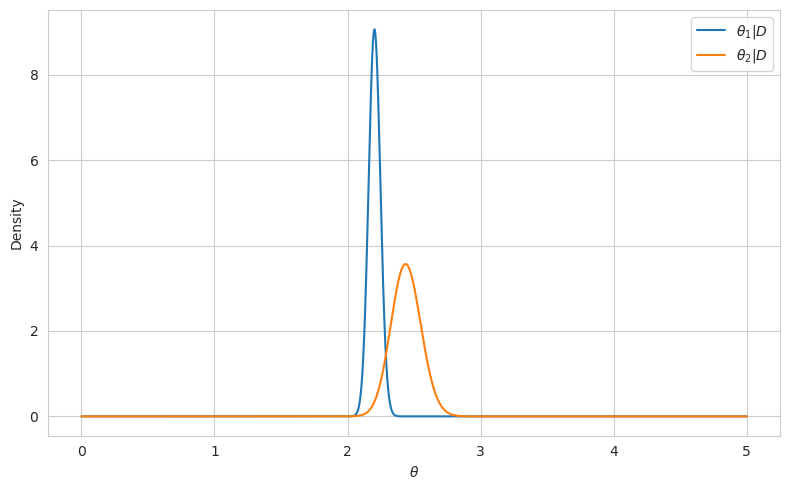
\includegraphics[width=0.575\textwidth]{4.5.c.1.png}
  \captionsetup{justification=centering}
  \caption{
    Posteriors with $a_1=a_2=2.2\times100\,, b_1=b_2=100$. \\
    $\mathbb{E}[\theta_1|D]=2.2$, $\mathbb{E}[\theta_1|D]=2.44$.
    95\% CI for $\theta_1$ is $[2.12, 2.29]$ and for $\theta_2$ is $[2.23, 2.67]$.
    $P[\theta_2 > \theta_1|D]=0.978$
  }
\end{figure*}

\begin{figure*}[!h]
  \centering
  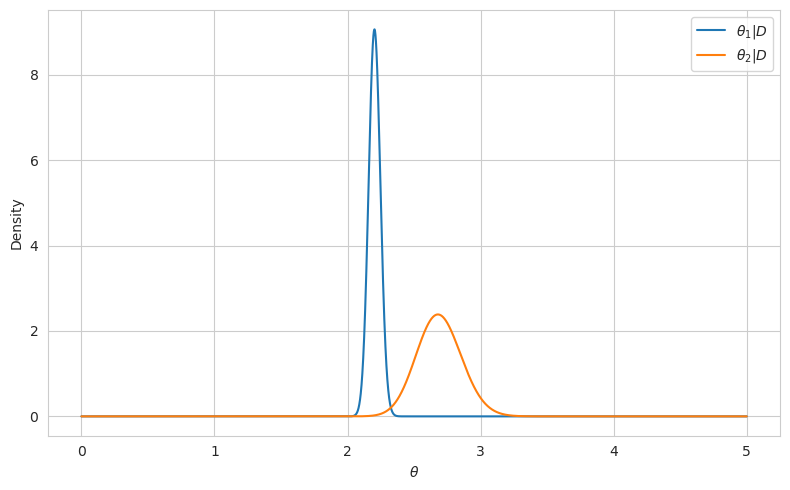
\includegraphics[width=0.575\textwidth]{4.5.c.2.png}
  \captionsetup{justification=centering}
  \caption{
    Posteriors with $a_1=2.2\times100\,, b_1=100\,, a_2=2.2\,, b_2=1$. \\
    $\mathbb{E}[\theta_1|D]=2.20$, $\mathbb{E}[\theta_1|D]=2.90$.
    95\% CI for $\theta_1$ is $[2.12, 2.29]$ and for $\theta_2$ is $[2.37, 3.03]$.
    $P[\theta_2 > \theta_1|D]=0.998$
  }
\end{figure*}

\begin{figure*}[!h]
  \centering
  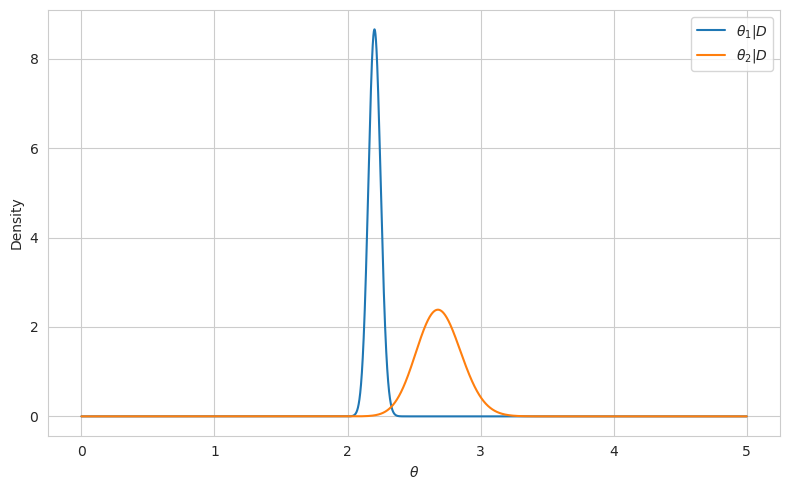
\includegraphics[width=0.575\textwidth]{4.5.c.3.png}
  \captionsetup{justification=centering}
  \caption{
    Posteriors with $a_1==a_2=2.2\,, b_1=b_2=1$. \\
    $\mathbb{E}[\theta_1|D]=2.20$, $\mathbb{E}[\theta_1|D]=2.689$.
    95\% CI for $\theta_1$ is $[2.114, 2.295]$ and for $\theta_2$ is $[2.371, 3.027]$.
    $P[\theta_2 > \theta_1|D]=0.998$
  }
\end{figure*}

\paragraph{(d)}
I think the assumption that the fatality rate has no relationship with the population size is reasonable. I don't see why a higher or lower population would result in differences in cancer rates. Although, perhaps the location of the reactor correlates with population. Nevertheless, if we assume a relationship between the two, we can model $Y_i$ with something similar to $Poisson(f(\theta, X_i))$. Or we can segment the population into multiple groups and assign $\theta$ priors differently by the segment and reactor.

\paragraph{(e)}
We can potentially create a hierarchical model. Establishing an assumption that both $\theta$ come from one parent distribution by modeling the $a$ and $b$ with a pooled prior. For instance, by putting a prior on $a$ and $b$, we assumes that $a_1$ and $a_2$ are generated from a parent distribution. Same for $b_1$ and $b_2$.


\section{Exercise 4.6}
We can see the induced log-odd distribution $\gamma$ below. Not surprising, $\gamma$ is not an uninformative prior. By imposing a uniform $\theta$ probability, we assume a log-odd ratio distribution centered around 0 and diffuses wildly to negative and positive infinity on both tails.

\begin{figure*}[!h]
  \centering
  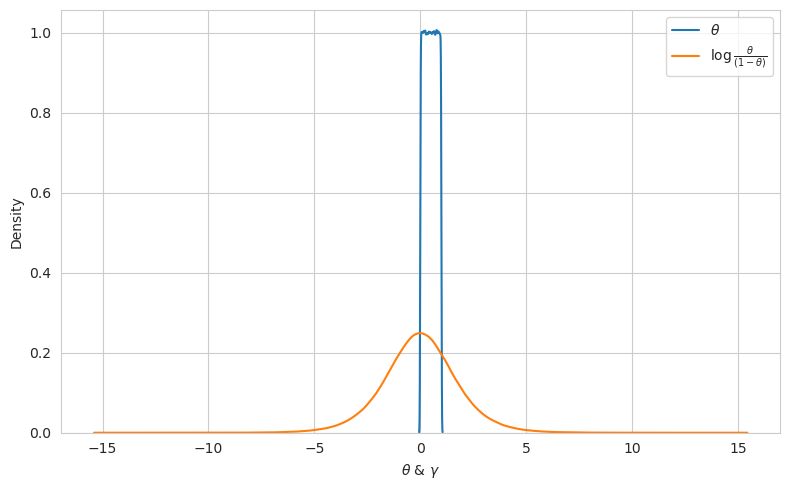
\includegraphics[width=0.7\textwidth]{4.6.png}
  \captionsetup{justification=centering}
  \caption{Comparison between the uniform $\theta$ and its induced log-odd $\gamma$}
\end{figure*}


\end{document}